% THIS DOCUMENT IS TAILORED TO REQUIREMENTS FOR SCIENTIFIC COMPUTING.  IT SHOULDN'T
% BE USED FOR NON-SCIENTIFIC COMPUTING PROJECTS
\documentclass[12pt]{article}

\usepackage{amsmath, mathtools}
\usepackage{amsfonts}
\usepackage{amssymb}
\usepackage{graphicx}
\usepackage{colortbl}
\usepackage{xr}
\usepackage{hyperref}
\usepackage{longtable}
\usepackage{xfrac}
\usepackage{tabularx}
\usepackage{float}
\usepackage{siunitx}
\usepackage{booktabs}
\usepackage{caption}
\usepackage{pdflscape}
\usepackage{afterpage}

\usepackage[round]{natbib}

%\usepackage{refcheck}

\hypersetup{
    bookmarks=true,         % show bookmarks bar?
      colorlinks=true,       % false: boxed links; true: colored links
    linkcolor=red,          % color of internal links (change box color with linkbordercolor)
    citecolor=green,        % color of links to bibliography
    filecolor=magenta,      % color of file links
    urlcolor=cyan           % color of external links
}

%% Comments

\usepackage{color}

\newif\ifcomments\commentstrue %displays comments
%\newif\ifcomments\commentsfalse %so that comments do not display

\ifcomments
\newcommand{\authornote}[3]{\textcolor{#1}{[#3 ---#2]}}
\newcommand{\todo}[1]{\textcolor{red}{[TODO: #1]}}
\else
\newcommand{\authornote}[3]{}
\newcommand{\todo}[1]{}
\fi

\newcommand{\wss}[1]{\authornote{blue}{SS}{#1}} 
\newcommand{\plt}[1]{\authornote{magenta}{TPLT}{#1}} %For explanation of the template
\newcommand{\an}[1]{\authornote{cyan}{Author}{#1}}

%% Common Parts

\newcommand{\progname}{OCRacle} % PUT YOUR PROGRAM NAME HERE
\newcommand{\authname}{Phillip Tran} % AUTHOR NAMES                  

\usepackage{hyperref}
    \hypersetup{colorlinks=true, linkcolor=blue, citecolor=blue, filecolor=blue,
                urlcolor=blue, unicode=false}
    \urlstyle{same}
                                


% For easy change of table widths
\newcommand{\colZwidth}{1.0\textwidth}
\newcommand{\colAwidth}{0.13\textwidth}
\newcommand{\colBwidth}{0.82\textwidth}
\newcommand{\colCwidth}{0.1\textwidth}
\newcommand{\colDwidth}{0.05\textwidth}
\newcommand{\colEwidth}{0.8\textwidth}
\newcommand{\colFwidth}{0.17\textwidth}
\newcommand{\colGwidth}{0.5\textwidth}
\newcommand{\colHwidth}{0.28\textwidth}

% Used so that cross-references have a meaningful prefix
\newcounter{defnum} %Definition Number
\newcommand{\dthedefnum}{GD\thedefnum}
\newcommand{\dref}[1]{GD\ref{#1}}
\newcounter{datadefnum} %Datadefinition Number
\newcommand{\ddthedatadefnum}{DD\thedatadefnum}
\newcommand{\ddref}[1]{DD\ref{#1}}
\newcounter{theorynum} %Theory Number
\newcommand{\tthetheorynum}{TM\thetheorynum}
\newcommand{\tref}[1]{TM\ref{#1}}
\newcounter{tablenum} %Table Number
\newcommand{\tbthetablenum}{TB\thetablenum}
\newcommand{\tbref}[1]{TB\ref{#1}}
\newcounter{assumpnum} %Assumption Number
\newcommand{\atheassumpnum}{A\theassumpnum}
\newcommand{\aref}[1]{A\ref{#1}}
\newcounter{goalnum} %Goal Number
\newcommand{\gthegoalnum}{GS\thegoalnum}
\newcommand{\gsref}[1]{GS\ref{#1}}
\newcounter{instnum} %Instance Number
\newcommand{\itheinstnum}{IM\theinstnum}
\newcommand{\iref}[1]{IM\ref{#1}}
\newcounter{reqnum} %Requirement Number
\newcommand{\rthereqnum}{R\thereqnum}
\newcommand{\rref}[1]{R\ref{#1}}
\newcounter{nfrnum} %NFR Number
\newcommand{\rthenfrnum}{NFR\thenfrnum}
\newcommand{\nfrref}[1]{NFR\ref{#1}}
\newcounter{lcnum} %Likely change number
\newcommand{\lthelcnum}{LC\thelcnum}
\newcommand{\lcref}[1]{LC\ref{#1}}
\newcounter{ucnum} %Unlikely change number
\newcommand{\ltheucnum}{UC\theucnum}
\newcommand{\ucref}[1]{UC\ref{#1}}

\usepackage{fullpage}

\newcommand{\deftheory}[9][Not Applicable]
{
\newpage
\noindent \rule{\textwidth}{0.5mm}

\paragraph{RefName: } \textbf{#2} \phantomsection 
\label{#2}

\paragraph{Label:} #3

\noindent \rule{\textwidth}{0.5mm}

\paragraph{Equation:}

#4

\paragraph{Description:}

#5

\paragraph{Notes:}

#6

\paragraph{Source:}

#7

\paragraph{Ref.\ By:}

#8

\paragraph{Preconditions for \hyperref[#2]{#2}:}
\label{#2_precond}

#9

\paragraph{Derivation for \hyperref[#2]{#2}:}
\label{#2_deriv}

#1

\noindent \rule{\textwidth}{0.5mm}

}

\begin{document}

\title{Software Requirements Specification for \progname: Latin Alphabet Character Recognition} 
\author{\authname}
\date{\today}
	
\maketitle

~\newpage

\pagenumbering{roman}

\tableofcontents

~\newpage

\section*{Revision History}

\begin{tabularx}{\textwidth}{p{3cm}p{2cm}X}
\toprule {\bf Date} & {\bf Version} & {\bf Notes}\\
\midrule
January 27, 2025 & 1.0 & Initial document creation \\
April 6, 2025 & 2.0 & Addressed feedback from Dr. Spencer Smith and Hussein Saad\\
\bottomrule
\end{tabularx}

~\\
% \plt{This template is intended for use by CAS 741.  For CAS 741 the template
% should be used exactly as given, except the Reflection Appendix can be deleted.
% For the capstone course it is a source of ideas, but shouldn't be followed
% exactly.  The exception is the reflection appendix.  All capstone SRS documents
% should have a reflection appendix.}

~\newpage

\section{Reference Material}

This section records information for easy reference.

\subsection{Table of Units}

This document does not use SI (Syst\`{e}me International d'Unit\'{e}s) as the
unit system because the problem domain is not a physical system.
~\newline

% Throughout this document SI (Syst\`{e}me International d'Unit\'{e}s) is employed
% as the unit system.  In addition to the basic units, several derived units are
% used as described below.  For each unit, the symbol is given followed by a
% description of the unit and the SI name.
% ~\newline

% \renewcommand{\arraystretch}{1.2}
% %\begin{table}[ht]
%   \noindent \begin{tabular}{l l l} 
%     \toprule		
%     \textbf{symbol} & \textbf{unit} & \textbf{SI}\\
%     \midrule 
%     px & pixel & N/A \\
%     \bottomrule
%   \end{tabular}
%   %	\caption{Provide a caption}
% %\end{table}

% \plt{Only include the units that your SRS actually uses.}

% \plt{Derived units, like newtons, pascal, etc, should show their derivation
%     (the units they are derived from) if their constituent units are in the
%     table of units (that is, if the units they are derived from are used in the
%     document).  For instance, the derivation of pascals as
%     $\si{\pascal}=\si{\newton\per\square\meter}$ is shown if newtons and m are
%     both in the table.  The derivations of newtons would not be shown if kg and
%     s are not both in the table.}

% \plt{The symbol for units named after people use capital letters, but the name
%   of the unit itself uses lower case.  For instance, pascals use the symbol Pa,
%   watts use the symbol W, teslas use the symbol T, newtons use the symbol N,
%   etc.  The one exception to this is degree Celsius.  Details on writing metric
%   units can be found on the 
%   \href{https://www.nist.gov/pml/weights-and-measures/writing-metric-units}
%   {NIST} web-page.}

\subsection{Table of Symbols}

The table that follows summarizes the symbols used in this document along with
their units. The symbols are listed in alphabetical order.

\renewcommand{\arraystretch}{1.2}
%\noindent \begin{tabularx}{1.0\textwidth}{l l X}
\noindent \begin{longtable*}{l l p{12cm}} \toprule
\textbf{symbol} & \textbf{unit} & \textbf{description}\\
\midrule
$I_{n \times m}$ & N/A & Matrix representing an input image of n rows
and m columns provided by the end user
\\
${L}$ & N/A & The number of distinct labels that the model can predict
\\
$P_{1 \times 26}$ & N/A & Probability vector representing the output of the
model, with ${L}$ columns representing the probability of each character
\\
$P_{pred}$ & N/A & The character predicted by the model.
\\ 
$T_{w \times w}$ & N/A & Matrix representing a ${w \times w}$ pixel image from
the training data provided by the technical user
\\
$g_t$ & N/A & The gradient of the cost function with respect to the weights at
time t
\\
$m_t$ & N/A & In the context of the Adam optimization algorithm, the first
moment estimate at time t
\\
$t$ & N/A & In the context of the Adam optimization algorithm, the time step
\\
$v_t$ & N/A & In the context of the Adam optimization algorithm, the second
moment estimate at time t
\\
$w$ & N/A & The number of rows/columns in the training dataset image
\\
$\alpha$ & N/A & Learning rate for the model
\\
$\epsilon$ & N/A & Small value to prevent division by zero
\\
$\theta$ & N/A & Vector representing the weights of the model
\\
$\hat{y}_i$ & N/A & The predicted probability of character i
\\
$y_i$ & N/A & The actual probability of character i
\\
\bottomrule
\end{longtable*}

% \plt{Use your problems actual symbols.  The si package is a good idea to use for
%   units.}

\subsection{Abbreviations and Acronyms}

\renewcommand{\arraystretch}{1.2}
\begin{tabular}{l l} 
  \toprule		
  \textbf{symbol} & \textbf{description}\\
  \midrule 
  A & Assumption\\
  DD & Data Definition\\
  GD & General Definition\\
  GS & Goal Statement\\
  IM & Instance Model\\
  LC & Likely Change\\
  PS & Physical System Description\\
  R & Requirement\\
  SRS & Software Requirements Specification\\
  \progname{} & Name of the Project\\
  TM & Theoretical Model\\
  \bottomrule
\end{tabular}\\

% \plt{Add any other abbreviations or acronyms that you add}

% \subsection{Mathematical Notation}

% \plt{This section is optional, but should be included for projects that make use
%   of notation to convey mathematical information.  For instance, if typographic
%   conventions (like bold face font) are used to distinguish matrices, this
%   should be stated here.  If symbols are used to show mathematical operations,
%   these should be summarized here.  In some cases the easiest way to summarize
%   the notation is to point to a text or other source that explains the
%   notation.}

% \plt{This section was added to the template because some students use very
%   domain specific notation.  This notation will not be readily understandable to
%   people outside of your domain.  It should be explained.}

\newpage

\pagenumbering{arabic}

% \plt{This SRS template is based on \citet{SmithAndLai2005, SmithEtAl2007,
%   SmithAndKoothoor2016}.  It will get you started.  You should not modify the
%   section headings, without first discussing the change with the course
%   instructor.  Modification means you are not following the template, which
%   loses some of the advantage of a template, especially standardization.
%   Although the bits shown below do not include type information, you may need to
%   add this information for your problem.  If you are unsure, please can ask the
%   instructor.}

% \plt{Feel free to change the appearance of the report by modifying the LaTeX
%   commands.}

% \plt{This template document assumes that a single program is being documented.
%   If you are documenting a family of models, you should start with a comm
%   onality
%   analysis.  A separate template is provided for this.  For program
%   families you should look at \cite{Smith2006, SmithMcCutchanAndCarette2017}.
%   Single family member programs are often programs based on a single physical
%   model.  General purpose tools are usually documented as a family.  Families of
%   physical models also come up.}

% \plt{The SRS is not generally written, or read, sequentially.  The SRS is a
%   reference document.  It is generally read in an ad hoc order, as the need
%   arises.  For writing an SRS, and for reading one for the first time, the
%   suggested order of sections is:
% \begin{itemize}
% \item Goal Statement
% \item Instance Models
% \item Requirements
% \item Introduction
% \item Specific System Description
% \end{itemize}
% }

% \plt{Guiding principles for the SRS document:
% \begin{itemize}
% \item Do not repeat the same information at the same abstraction level.  If
%   information is repeated, the repetition should be at a different abstraction
%   level.  For instance, there will be overlap between the scope section and the
%   assumptions, but the scope section will not go into as much detail as the
%   assumptions section.
% \end{itemize}
% }

% \plt{The template description comments should be disabled before submitting this
%   document for grading.}

% \plt{You can borrow any wording from the text given in the template.  It is part
%   of the template, and not considered an instance of academic integrity.  Of
%   course, you need to cite the source of the template.}

% \plt{When the documentation is done, it should be possible to trace back to the
%   source of every piece of information.  Some information will come from
%   external sources, like terminology.  Other information will be derived, like
%   General Definitions.}

% \plt{An SRS document should have the following qualities: unambiguous,
%   consistent, complete, validatable, abstract and traceable.}

% \plt{The overall goal of the SRS is that someone that meets the Characteristics
%   of the Intended Reader (Section~\ref{sec_IntendedReader}) can learn,
%   understand and verify the captured domain knowledge.  They should not have to
%   trust the authors of the SRS on any statements.  They should be able to
%   independently verify/derive every statement made.}

\section{Introduction}

Researchers analyzing physical print documents such as newspapers, books, and
letters often need a means of digitizing the text in these documents. This
enables them to search and analyze the text data more efficiently. Especially in
the case of historical documents, digitizing the text can help preserve the
information contained in these documents.

Optical Character Recognition (OCR) is a technology that allows for the
extraction of text information from scanned documents, images, and other optical
formats where text may be present. This digitalization process enables
researchers to use computer programs to find trends and patterns in the
digitized text.

The \progname{} project aims to develop a program that can recognize and
classify a single Latin alphabet character in an image.

The following section describes the purpose of the document, the scope of
requirements, characteristics of the intended reader, and the organizational
roadmap of the document.

% \plt{The introduction section is written to introduce the problem.  It starts
%   general and focuses on the problem domain. The general advice is to start with
% a paragraph or two that describes the problem, followed by a ``roadmap''
% paragraph.  A roadmap orients the reader by telling them what sub-sections to
% expect in the Introduction section.}

\subsection{Purpose of Document}

This document serves as a software requirements specification for the \progname{}
project. This includes the general system description, problem description,
solution characteristics, and requirements. This document will be used a
reference for building the solution.

% \plt{This section summarizes the purpose of the SRS document.  It does not focus
%   on the problem itself.  The problem is described in the ``Problem
%   Description'' section (Section~\ref{Sec_pd}).  The purpose is for the document
%   in the context of the project itself, not in the context of this course.
%   Although the ``purpose'' of the document is to get a grade, you should not
%   mention this.  Instead, ``fake it'' as if this is a real project.  The purpose
%   section will be similar between projects.  The purpose of the document is the
%   purpose of the SRS, including communication, planning for the design stage,
%   etc.}

\subsection{Scope of Requirements} 

This program is intended for classifying a single handwritten Latin alphabet
character in an image. Handwritten cursive characters are not an expected input
of this program.

% \textsc{\plt{Modelling the real world requires simplification.  The full complexity of
%   the actual physics, chemistry, biology is too much for existing models, and
%   for existing computational solution techniques.  Rather than say what is in
%   the scope, it is usually easier to say what is not.  You can think of it as
%   the scope is initially everything, and then it is constrained to create the
%   actual scope.  For instance, the problem can be restricted to 2 dimensions, or
%   it can ignore the effect of temperature (or pressure) on the material
%   properties, etc.}  

% \plt{The scope section is related to the assumptions section
%   (Section~\ref{sec_assumpt}).  However, the scope and the assumptions are not
%   at the same level of abstraction.  The scope is at a high level.  The focus is
%   on the ``big picture'' assumptions.  The assumptions section lists, and
%   describes, all of the assumptions.}

% \plt{The scope section is relevant for later determining typical values of inputs. The scope should make it clear what inputs are reasonable to expect. This is a distinction between scope and context (context is a later section).  Scope affects the inputs while context affects how the software will be used.}
% }
\subsection{Characteristics of Intended Reader} \label{sec_IntendedReader}

The intended reader of this document should have knowledge equivalent to the
following coursework:

\begin{itemize}
  \item MATH 1B03: Linear Algebra
  \item COMPSCI 4ML3: Introduction to Machine Learning
\end{itemize}

% \plt{This section summarizes the skills and knowledge of the readers of the
%   SRS.  It does NOT have the same purpose as the ``User Characteristics''
%   section (Section~\ref{SecUserCharacteristics}).  The intended readers are the
%   people that will read, review and maintain the SRS.  They are the people that
%   will conceivably design the software that is intended to meet the
%   requirements.  The user, on the other hand, is the person that uses the
%   software that is built.  They may never read this SRS document.  Of course,
%   the same person could be a ``user'' and an ``intended reader.''}

% \plt{The intended reader characteristics should be written as unambiguously and
%   as specifically as possible.  Rather than say, the user should have an
%   understanding of physics, say what kind of physics and at what level.  For
%   instance, is high school physics adequate, or should the reader have had a
%   graduate course on advanced quantum mechanics?}

\subsection{Organization of Document}

After the brief introduction, the document details the general system
description, problem description, solutions characteristic specification, and
requirements.

% \plt{This section provides a roadmap of the SRS document.  It will help the
%   reader orient themselves.  It will provide direction that will help them
%   select which sections they want to read, and in what order.  This section will
%   be similar between project.}

\section{General System Description}

This section provides general information about the system.  It identifies the
interfaces between the system and its environment, describes the user
characteristics and lists the system constraints.

\subsection{System Context}

% \plt{Your system context will include a figure that shows the abstract view of
%   the software.  Often in a scientific context, the program can be viewed
%   abstractly following the design pattern of Inputs $\rightarrow$ Calculations
%   $\rightarrow$ Outputs.  The system context will therefore often follow this
%   pattern.  The user provides inputs, the system does the calculations, and then
%   provides the outputs to the user.  The figure should not show all of the
%   inputs, just an abstract view of the main categories of inputs (like material
%   properties, geometry, etc.).  Likewise, the outputs should be presented from
%   an abstract point of view.  In some cases the diagram will show other external
%   entities, besides the user.  For instance, when the software product is a
%   library, the user will be another software program, not an actual end user.
%   If there are system constraints that the software must work with external
%   libraries, these libraries can also be shown on the System Context diagram.
%   They should only be named with a specific library name if this is required by
%   the system constraint.}

We can take two perspectives on the system context. The first is the technical
user, who interfaces with the \progname{} program to produce a model that can
predict the character in an image. The second is the end user, who uses the
\progname{} model to predict the character in an input image.

\begin{figure}[h!]
  \begin{center}
    \includegraphics[page=2, width=0.6\textwidth]{SystemContextFigure}
    \caption{System Context of End User}
    \label{Fig_SystemContext2} 
  \end{center}
\end{figure}


\begin{itemize}
  \item Technical User Responsibilities:
  \begin{itemize}
  \item Provide an image dataset to train the model following A\ref{A_EMNIST}, A\ref{A_Latin}, and A\ref{A_Preprocessing}.
  \end{itemize}
  \item \progname{} Responsibilities:
  \begin{itemize}
  \item Detect incompatible input.
  \item Train the model on the image dataset provided by the user.
  \item Output a trained model that can predict the character in an image.
  \end{itemize}
  \end{itemize}

\begin{figure}[h!]
  \begin{center}
    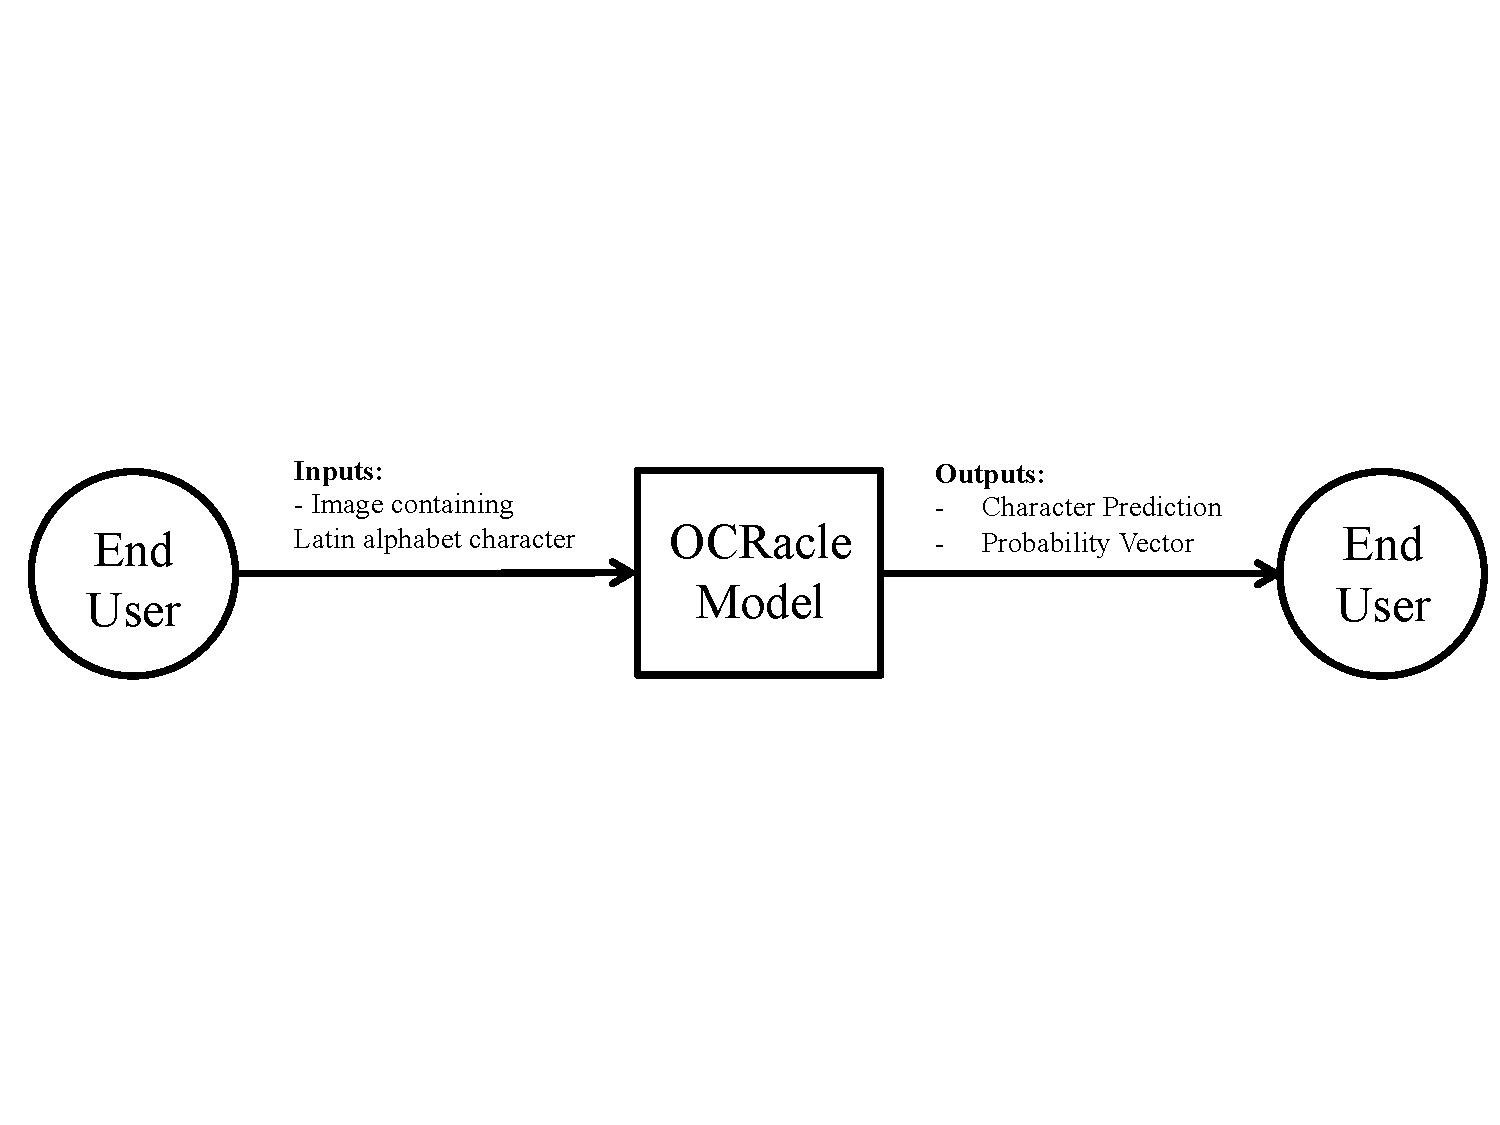
\includegraphics[page=1, width=0.6\textwidth]{SystemContextFigure}
    \caption{System Context of Technical User}
    \label{Fig_SystemContext1} 
  \end{center}
\end{figure}

% \plt{For each of the entities in the system context diagram its responsibilities
%   should be listed.  Whenever possible the system should check for data quality,
%   but for some cases the user will need to assume that responsibility.  The list
%   of responsibilities should be about the inputs and outputs only, and they
%   should be abstract.  Details should not be presented here.  However, the
%   information should not be so abstract as to just say ``inputs'' and
%   ``outputs''.  A summarizing phrase can be used to characterize the inputs.
%   For instance, saying ``material properties'' provides some information, but it
%   stays away from the detail of listing every required properties.}

\begin{itemize}
\item End User Responsibilities:
\begin{itemize}
\item Provide an image following A\ref{A_Preprocessing}.
\item Run the program on a compatible platform.
\item Interface with the program.
\end{itemize}
\item \progname{} Responsibilities:
\begin{itemize}
\item Detect incompatible input.
\item Provide an interface to view the predicted character.
\item Provide an interface to view the probability distribution.
\end{itemize}
\end{itemize}

% \plt{Identify in what context the software will typically be used.  Is it for
% exploration? education? engineering work? scientific work?. Identify whether it
% will be used for mission-critical or safety-critical applications.} \plt{This
% additional context information is needed to determine how much effort should be
% devoted to the rationale section.  If the application is safety-critical, the
% bar is higher.  This is currently less structured, but analogous to, the idea to
% the Automotive Safety Integrity Levels (ASILs) that McSCert uses in their
% automotive hazard analyses.}

\subsection{User Characteristics} \label{SecUserCharacteristics}

Both the technical user and the end user of \progname{} should have an a basic
understanding of the command line to setup the program. At a minimum, the users
should have the knowledge contained within the \href{https://missing.csail.mit.edu/}{MIT Missing Semester} course.

The provided user manual should be approachable for users of this skill level
and allow them to train and use the model effectively, even if they are not
familiar with the technical details of the program.

% \plt{This section summarizes the knowledge/skills expected of the user.
%   Measuring usability, which is often a required non-function requirement,
%   requires knowledge of a typical user.  As mentioned above, the user is a
%   different role from the ``intended reader,'' as given in
%   Section~\ref{sec_IntendedReader}.  As in Section~\ref{sec_IntendedReader}, the
%   user characteristics should be specific an unambiguous.  For instance, ``The
%   end user of \progname{} should have an understanding of undergraduate Level 1
%   Calculus and Physics.''}

\subsection{System Constraints}

The input image must contain a single Latin alphabet character. The system
will be unable to identify multiple characters in a single image. It will also
be unable to determine if there are no identifiable characters in the image.

\section{Specific System Description}

This section first presents the problem description, which gives a high-level
view of the problem to be solved.  This is followed by the solution
characteristics specification, which presents the assumptions, theories,
definitions and finally the instance models.

% \plt{Add any project specific details that are relevant for the section overview.}

\subsection{Problem Description} \label{Sec_pd}

\progname{} is intended to solve the problem of extracting text information from
a scanned document, image, and other optical formats where text may be present,
such that this textual data can be used for further analysis.

\subsubsection{Terminology and  Definitions}

% \plt{This section is expressed in words, not with equations.  It provide the
%   meaning of the different words and phrases used in the domain of the problem.
% The terminology is used to introduce concepts from the world outside of the
% mathematical model  The terminology provides a real world connection to give the
% mathematical model meaning.}

This subsection provides a list of terms that are used in the subsequent
sections and their meaning, with the purpose of reducing ambiguity and making it
easier to correctly understand the requirements:

\begin{itemize}

\item \textbf{OCR:} Optical Character Recognition, the process of extracting text
\item \textbf{EMNIST:} Extended MNIST, a dataset of handwritten characters
\item \textbf{Latin Alphabet:} The alphabet used in the English language
\item \textbf{Character:} A single letter in the Latin alphabet
\item \textbf{Image:} A 2D array of pixel values
\item \textbf{Pixel:} The smallest unit of a digital image
\item \textbf{Probability Vector:} A vector representing the likelihood of each character
\item \textbf{Model:} A trained machine learning model
\item \textbf{Prediction:} The output of the model
\item \textbf{Preprocessing:} The process of preparing the image for input into the model
\item \textbf{Label:} The correct character associated with an image
\item \textbf{Training:} The process of teaching the model to predict characters
\item \textbf{Training Data:} The dataset used to train the model
\item \textbf{Downsampling:} The process of reducing the dimensions of an image by removing pixels while preserving the important features of the image

\end{itemize}

\subsubsection{Physical System Description} \label{sec_phySystDescrip}

% \plt{The purpose of this section is to clearly and unambiguously state the
%   physical system that is to be modelled. Effective problem solving requires a
%   logical and organized approach. The statements on the physical system to be
%   studied should cover enough information to solve the problem. The physical
%   description involves element identification, where elements are defined as
%   independent and separable items of the physical system. Some example elements
%   include acceleration due to gravity, the mass of an object, and the size and
%   shape of an object. Each element should be identified and labelled, with their
%   interesting properties specified clearly. The physical description can also
%   include interactions of the elements, such as the following: i) the
%   interactions between the elements and their physical environment; ii) the
%   interactions between elements; and, iii) the initial or boundary conditions.}

% \plt{The elements of the physical system do not have to correspond to an actual
% physical entity.  They can be conceptual.  This is particularly important when
% the documentation is for a numerical method. }

The physical system of \progname{}, as shown in Figure \ref{Fig_PhysicalSystem},
includes the following elements:

\begin{itemize}

\item[PS1:] For training the model, the system requires a dataset of images of
Latin alphabet characters, alongside a corresponding label for each image.
\item[PS2:] For using the model as an end user, the system requires an image
of a single Latin alphabet character.

\end{itemize}

% \plt{A figure here makes sense for most SRS documents}

\begin{figure}[h!]
\begin{center}
{
  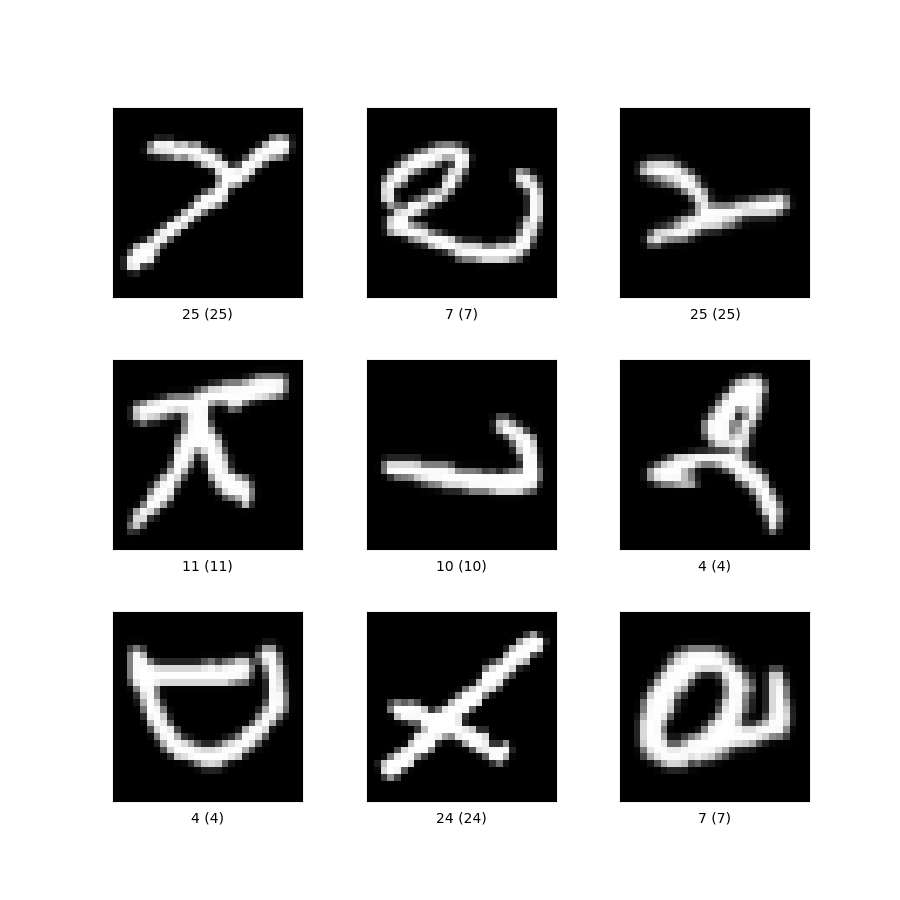
\includegraphics[width=0.5\textwidth]{emnist-letters-3.1.0.png}
}
\caption{\label{Fig_PhysicalSystem} A sample of the EMNIST dataset,
representing the Latin alphabet}
\end{center}
\end{figure}

\subsubsection{Goal Statements}

% \plt{The goal statements refine the ``Problem Description''
%   (Section~\ref{Sec_pd}).  A goal is a functional objective the system under
%   consideration should achieve. Goals provide criteria for sufficient
%   completeness of a requirements specification and for requirements
%   pertinence. Goals will be refined in Section “Instanced Models”
%   (Section~\ref{sec_instance}). Large and complex goals should be decomposed
%   into smaller sub-goals.  The goals are written abstractly, with a minimal
%   amount of technical language.  They should be understandable by non-domain
%   experts.}

\noindent Given the training data provided by the technical user, the goal
statements are:

\begin{itemize}

\item[GS\refstepcounter{goalnum}\thegoalnum \label{G_train}:] Produce a trained
model that can predict the character in an image.

\end{itemize}

\noindent Given an image containing a single Latin alphabet character from the
end user, the goal statements are:

\begin{itemize}

\item[GS\refstepcounter{goalnum}\thegoalnum \label{G_predict}:] Predict the character.
\item[GS\refstepcounter{goalnum}\thegoalnum \label{G_probability}:] Produce a probability distribution
representing the likelihood of each character.

\end{itemize}

\subsection{Solution Characteristics Specification}

This section specifies the information in the solution domain of the system
to be developed. This section is intended to express what is required in
such a way that analysts and stakeholders get a clear picture, and the
latter will accept it. The purpose of this section is to reduce the problem
into one expressed in mathematical terms. Mathematical expertise is used to
extract the essentials from the underlying physical description of the
problem, and to collect and substantiate all physical data pertinent to the
problem.

% \plt{This section presents the solution characteristics by successively refining
%   models.  It starts with the abstract/general Theoretical Models (TMs) and
%   refines them to the concrete/specific Instance Models (IMs).  If necessary
%   there are intermediate refinements to General Definitions (GDs).  All of these
%   refinements can potentially use Assumptions (A) and Data Definitions (DD).
%   TMs are refined to create new models, that are called GMs or IMs. DDs are not
%   refined; they are just used. GDs and IMs are derived, or refined, from other
%   models. DDs are not derived; they are just given. TMs are also just given, but
%   they are refined, not used.  If a potential DD includes a derivation, then
%   that means it is refining other models, which would make it a GD or an IM.}

% \plt{The above makes a distinction between ``refined'' and ``used.'' A model is
%   refined to another model if it is changed by the refinement. When we change a
%   general 3D equation to a 2D equation, we are making a refinement, by applying
%   the assumption that the third dimension does not matter. If we use a
%   definition, like the definition of density, we aren't refining, or changing
%   that definition, we are just using it.}

% \plt{The same information can be a TM in one problem and a DD in another.  It is
%   about how the information is used.  In one problem the definition of
%   acceleration can be a TM, in another it would be a DD.}

% \plt{There is repetition between the information given in the different chunks
%   (TM, GDs etc) with other information in the document.  For instance, the
%   meaning of the symbols, the units etc are repeated.  This is so that the
%   chunks can stand on their own when being read by a reviewer/user.  It also
%   facilitates reuse of the models in a different context.}

The relationships between the parts of the document are show in
the following figure.  In this diagram ``may ref'' has the same role as
``uses'' above.  The figure adds ``Likely Changes,'' which are able to
reference (use) Assumptions.

\begin{figure}[H]
  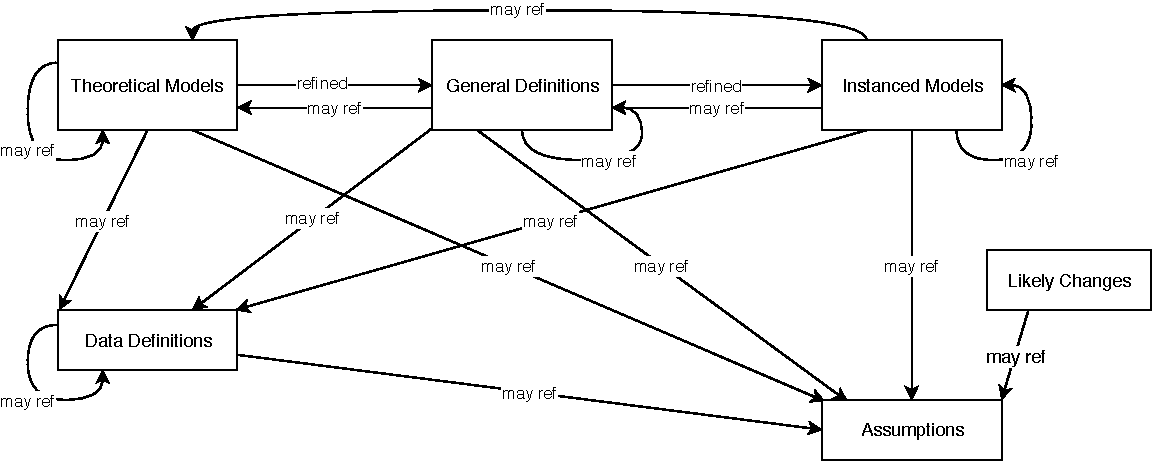
\includegraphics[scale=0.9]{RelationsBetweenTM_GD_IM_DD_A.pdf}
\end{figure}

The instance models that govern \progname{} are presented in
Subsection~\ref{sec_instance}.  The information to understand the meaning of the
instance models and their derivation is also presented, so that the instance
models can be verified.

\subsubsection{Assumptions} \label{sec_assumpt}

% \plt{The assumptions are a refinement of the scope.  The scope is general, where
%   the assumptions are specific.  All assumptions should be listed, even those
%   that domain experts know so well that they are rarely (if ever) written down.}
% \plt{The document should not take for granted that the reader knows which
%   assumptions have been made. In the case of unusual assumptions, it is
%   recommended that the documentation either include, or point to, an explanation
%   and justification for the assumption.} 
% \plt{If it helps with the organization and understandability, the assumptions
% can be presented as sub sections.  The following sub-sections are options:
% background theory assumptions, helper theory assumptions, generic theory
% assumptions, problem specific assumptions, and rationale assumptions}

This section simplifies the original problem and helps in developing the
theoretical model by filling in the missing information for the physical system.
The numbers given in the square brackets refer to the theoretical model [TM],
general definition [GD], data definition [DD], instance model [IM], or likely
change [LC], in which the respective assumption is used.

\begin{itemize}

\item[A\refstepcounter{assumpnum}\theassumpnum \label{A_EMNIST}:] The model will be trained on the EMNIST letters dataset where each image is 28x28 pixels as required by IM\ref{IM_Training}. The dataset also treats uppercase and lowercase letters as the same character, so the model will be trained on both uppercase and lowercase letters.
\item[A\refstepcounter{assumpnum}\theassumpnum \label{A_Latin}:] The input images and training images will contain only a single Latin alphabet character per image, as required by IM\ref{IM_Training} and IM\ref{IM_CharacterPrediction}.
\item[A\refstepcounter{assumpnum}\theassumpnum \label{A_Preprocessing}:] All
input images from the user undergo preprocessing such that they are in the same
format as the training data, where TM\ref{TM:BI} and TM\ref{TM:N} are applied in
IM\ref{IM_PreProcessing}.

\end{itemize}

\subsubsection{Theoretical Models}\label{sec_theoretical}

% \plt{Theoretical models are sets of abstract mathematical equations or axioms
%   for solving the problem described in Section ``Physical System Description''
%   (Section~\ref{sec_phySystDescrip}). Examples of theoretical models are
%   physical laws, constitutive equations, relevant conversion factors, etc.}

% \plt{Optionally the theory section could be divided into subsections to provide
% more structure and improve understandability and reusability.  Potential
% subsections include the following: Context theories, background theories, helper
% theories, generic theories, problem specific theories, final theories and
% rationale theories.}

This section focuses on the general equations and laws that \progname{} is based
on. 

% \plt{Modify the examples below for your problem, and add additional models
%   as appropriate.}

~\newline

\refstepcounter{theorynum}\label{TM:BI}
\noindent
\deftheory
% #2 refname of theory
{TM:BI}
% #3 label
{Bicubic Interpolation}
% #4 equation
{
  $f(x, y) = \sum_{i=0}^{3} \sum_{j=0}^{3} a_{ij} x^i y^j$
}
% #5 description
{
  Bicubic interpolation is a method of interpolating data points on a 2D grid.
  The method uses a 4x4 grid of data points to estimate the value of a point
  within the grid. This is useful for downsampling an image from a higher
  resolution (e.g. 128x128) to a lower resolution (e.g. 28x28).
}
% #6 Notes
{
None.
}
% #7 Source
{
  \url{https://en.wikipedia.org/wiki/Bicubic_interpolation}
}
% #8 Referenced by
{
  A\ref{A_Preprocessing}
}
% #9 Preconditions
{
None
}
% #1 derivation - not applicable by default
{}

\refstepcounter{theorynum}\label{TM:N}
\noindent
\deftheory
% #2 refname of theory
{TM:N}
% #3 label
{Normalization}
% #4 equation
{
  $f(x) = 
  \begin{cases} 
  0, & \text{if } \max(X) = \min(X) \\
  \frac{x- \min(X)}{\max(X) - \min(X)}, & \text{otherwise}
  \end{cases}$
}
% #5 description
{
  Normalization is a method of scaling data to a fixed range. This is useful for
  ensuring that the input data to a machine learning model is within a certain
  range. For instance, the pixel values of an image are typically normalized to
  the range [0, 1], where 0 represents black and 1 represents white. We prevent
  a divide by zero case by checking if the minimum and maximum values are the
  same before performing the normalization.
}
% #6 Notes
{
None.
}
% #7 Source
{
  \url{https://en.wikipedia.org/wiki/Normalization_(image_processing)}
}
% #8 Referenced by
{
  A\ref{A_Preprocessing}, IM\ref{IM_PreProcessing}
}
% #9 Preconditions
{
None
}
% #1 derivation - not applicable by default
{}

\refstepcounter{theorynum}\label{TM:ADAM}
\noindent
\deftheory
% #2 refname of theory
{TM:ADAM}
% #3 label
{ADAM Optimization}
% #4 equation
{
  ~\newline
  $m_t = \beta_1 m_{t-1} + (1 - \beta_1) g_t$\\
  $v_t = \beta_2 v_{t-1} + (1 - \beta_2) g_t^2$\\
  $\hat{m}_t = \frac{m_t}{1 - \beta_1^t}$\\
  $\hat{v}_t = \frac{v_t}{1 - \beta_2^t}$\\
  $\theta_t = \theta_{t-1} - \alpha \frac{\hat{m}_t}{\sqrt{\hat{v}_t} + \epsilon}$
}
% #5 description
{
  ADAM Optimization is used to train machine learning models. ADAM stands for
  Adaptive Moment Estimation, which means that the algorithm adapts the learning
  rate during training.
  The algorithm uses the first and second moments ($m_t$ and $v_t$) of the
  gradients ($g_t$) to update the parameters $\theta_t$. The hyperparameters
  $\beta_1$, $\beta_2$, $\alpha$, and $\epsilon$ control the behavior of the
  algorithm. $\beta_1$ and $\beta_2$ control the exponential decay rates of the
  first and second moments, $\alpha$ is the learning rate, and $\epsilon$ is a
  small value to prevent division by zero.
}
% #6 Notes
{
None.
}
% #7 Source
{
  \cite{KigmaAndBa2014}
}
% #8 Referenced by
{
  IM\ref{IM_Training}, DD\ref{DD_LearningRate}, DD\ref{DD_Parameters}, DD\ref{DD_Gradient}
}
% #9 Preconditions
{
None
}
% #1 derivation - not applicable by default
{}

\refstepcounter{theorynum}\label{TM:CELF}
\noindent
\deftheory
% #2 refname of theory
{TM:CELF}
% #3 label
{Cross-Entropy Loss Function}
% #4 equation
{
  $L(y, \hat{y}) = -\sum_{i} y_i \log(\hat{y}_i)$
}
% #5 description
{
  The cross-entropy loss function is used to measure the difference between the
  predicted probability distribution $\hat{y}$ and the true probability
  distribution $y$. A greater loss is incurred when the predicted probability
  distribution is further from the true distribution. Heavier penalties occur
  when the prediction dictates there to be a near-equal likelihood that the true
  label could belong to multiple classes.
}
% #6 Notes
{
None.
}
% #7 Source
{
  \cite{Mao2023}
}
% #8 Referenced by
{
  A\ref{A_Preprocessing}, IM\ref{IM_Training}, DD\ref{DD_ProbabilityDistribution}, DD\ref{DD_TrueLabel}
}
% #9 Preconditions
{
None
}
% #1 derivation - not applicable by default
{}

% \plt{``Ref.\ By'' is used repeatedly with the different types of information.
%   This stands for Referenced By.  It means that the models, definitions and
%   assumptions listed reference the current model, definition or assumption.
%   This information is given for traceability.  Ref. By provides a pointer in the
%   opposite direction to what we commonly do.  You still need to have a reference
%   in the other direction pointing to the current model, definition or
%   assumption.  As an example, if TM1 is referenced by GD2, that means that GD2 will
%   explicitly include a reference to TM1.}

~\newline

\subsubsection{General Definitions}\label{sec_gendef}

% \plt{General Definitions (GDs) are a refinement of one or more TMs, and/or of
%   other GDs.  The GDs are less abstract than the TMs.  Generally the reduction
%   in abstraction is possible through invoking (using/referencing) Assumptions.
%   For instance, the TM could be Newton's Law of Cooling stated abstracting.  The
%   GD could take the general law and apply it to get a 1D equation.}

This section collects the laws and equations that will be used in building the
instance models.

% \plt{Some projects may not have any content for this section, but the section
%   heading should be kept.}  \plt{Modify the examples below for your problem, and
%   add additional definitions as appropriate.}

~\newline

\noindent
\begin{minipage}{\textwidth}
\renewcommand*{\arraystretch}{1.5}
\begin{tabular}{| p{\colAwidth} | p{\colBwidth}|}
\hline
\rowcolor[gray]{0.9}
Number& GD\refstepcounter{defnum}\thedefnum \label{GD_ReLU}\\
\hline
Label &\bf Rectified Linear Unit (ReLU)\\
\hline
SI Units& N/A\\
\hline
Equation&$f(x) = \max(0, x)$\\
\hline
Description &
The function returns 0 if $x$ is negative. Otherwise, the function will return
$x$. This function is used in neural networks as an activation function. An
activation function determines the output of a node in a neural network.
\\
\hline
Source & \cite{Bai2022}\\
\hline
Ref.\ By & GD\ref{GD_CNN} \\
\hline
\end{tabular}
\end{minipage}

~\newline

\noindent
\begin{minipage}{\textwidth}
\renewcommand*{\arraystretch}{1.5}
\begin{tabular}{| p{\colAwidth} | p{\colBwidth}|}
\hline
\rowcolor[gray]{0.9}
Number& GD\refstepcounter{defnum}\thedefnum \label{GD_SM}\\
\hline
Label &\bf Softmax\\
\hline
SI Units& N/A\\
\hline
Equation& $f(x)_i = \frac{e^{x_i}}{\sum_{j=1}^{n} e^{x_j}}$\\
\hline
Description &
The softmax function takes in a vector of $n$ real numbers and returns a vector
of the same length. The exponential function is applied to each element of the
input vector, and the resulting vector is divided by the sum of the exponential
values. This achieves a probability distribution over the input vector.
\\
\hline
Source & \cite{GaoAndPavel2018}\\
\hline
Ref.\ By & GD\ref{GD_CNN} \\
\hline
\end{tabular}
\end{minipage}\\


\noindent
\begin{minipage}{\textwidth}
\renewcommand*{\arraystretch}{1.5}
\begin{tabular}{| p{\colAwidth} | p{\colBwidth}|}
\hline
\rowcolor[gray]{0.9}
Number& GD\refstepcounter{defnum}\thedefnum \label{GD_CNN}\\
\hline
Label &\bf Convolutional Neural Network (CNN)\\
\hline
SI Units& N/A\\
\hline
Equation&
\begin{equation*}
\begin{aligned}
&\text{Convolutional Layer:} \\
&z = w \ast x + b \\
&a = \text{ReLU}(z) \\
&\text{Pooling Layer:} \\
&\text{Max Pooling: } a = \max(a) \\
&\text{Softmax Layer:} \\
&\hat{y} = \text{Softmax}(a)
\end{aligned}
\end{equation*}
\\
\hline
Description &
A Convolutional Neural Network (CNN) is a type of neural network that is
typically used for image classification tasks such as OCR. The network consists
of convolutional layers, pooling layers, and softmax layers. The convolutional
layer applies a filter to the input image, the pooling layer reduces the
dimensionality of the image, and the softmax layer produces a probability
distribution over the classes.
\\
\hline
Source & \cite{GuoEtAl2017}\\
\hline
Ref.\ By & IM\ref{IM_Training}, IM\ref{IM_CharacterPrediction}\\
\hline
\end{tabular}
\end{minipage}\\

% \subsubsection*{Detailed derivation of simplified rate of change of temperature}

% \plt{This may be necessary when the necessary information does not fit in the
%   description field.}
% \plt{Derivations are important for justifying a given GD.  You want it to be
%   clear where the equation came from.}

\subsubsection{Data Definitions}\label{sec_datadef}

% \plt{The Data Definitions are definitions of symbols and equations that are
%   given for the problem.  They are not derived; they are simply used by other
%   models.  For instance, if a problem depends on density, there may be a data
%   definition for the equation defining density.  The DDs are given information
%   that you can use in your other modules.}

% \plt{All Data Definitions should be used (referenced) by at least one other
%   model.}

This section collects and defines all the data needed to build the instance
models. The dimension of each quantity is also given. 

% \plt{Modify the examples
%   below for your problem, and add additional definitions as appropriate.}

~\newline

\noindent
\begin{minipage}{\textwidth}
\renewcommand*{\arraystretch}{1.5}
\begin{tabular}{| p{\colAwidth} | p{\colBwidth}|}
\hline
\rowcolor[gray]{0.9}
Number& DD\refstepcounter{datadefnum}\thedatadefnum \label{DD_InputImage}\\
\hline
Label& \bf Input Image\\
\hline
Symbol &$I_{n \times m}$\\
\hline
  SI Units & N/A\\
  \hline
  Equation& N/A\\
  \hline
  Description & 
  $I$ is a 2D array of pixel values representing an image. The image has $n$
  rows and $m$ columns. Each pixel value is an integer between 0 and 255.
  \\
  \hline
  Sources& N/A \\
  \hline
  Ref.\ By & IM\ref{IM_PreProcessing}, TM\ref{TM:BI}, TM\ref{TM:N}\\
  \hline
\end{tabular}
\end{minipage}\\

~\newline

\noindent
\begin{minipage}{\textwidth}
\renewcommand*{\arraystretch}{1.5}
\begin{tabular}{| p{\colAwidth} | p{\colBwidth}|}
\hline
\rowcolor[gray]{0.9}
Number& DD\refstepcounter{datadefnum}\thedatadefnum \label{DD_TrainingImage}\\
\hline
Label& \bf Training Image\\
\hline
Symbol &$I_{n \times m}$\\
\hline
  SI Units & N/A\\
  \hline
  Equation& N/A\\
  \hline
  Description & 
  $T$ is a 2D array of pixel values representing an image. The image has $n$
  rows and $m$ columns. Each pixel value is either 0 for black or 1 for white.
  \\
  \hline
  Sources& N/A \\
  \hline
  Ref.\ By & IM\ref{IM_Training}\\
  \hline
\end{tabular}
\end{minipage}\\

~\newline

\noindent
\begin{minipage}{\textwidth}
\renewcommand*{\arraystretch}{1.5}
\begin{tabular}{| p{\colAwidth} | p{\colBwidth}|}
\hline
\rowcolor[gray]{0.9}
Number& DD\refstepcounter{datadefnum}\thedatadefnum \label{DD_LearningRate}\\
\hline
Label& \bf Learning Rate\\
\hline
Symbol &$\alpha$\\
\hline
  SI Units & N/A\\
  \hline
  Equation& N/A\\
  \hline
  Description & 
  $\alpha$ is a hyperparameter that controls how much the model weights are
  updated during training. With a small learning rate, the model will learn
  slowly, but with a large learning rate, the model may never find the optimal
  solution.
  \\
  \hline
  Sources& \cite{KigmaAndBa2014} \\
  \hline
  Ref.\ By & IM\ref{IM_Training}, TM\ref{TM:ADAM}\\
  \hline
\end{tabular}
\end{minipage}\\

~\newline

\noindent
\begin{minipage}{\textwidth}
\renewcommand*{\arraystretch}{1.5}
\begin{tabular}{| p{\colAwidth} | p{\colBwidth}|}
\hline
\rowcolor[gray]{0.9}
Number& DD\refstepcounter{datadefnum}\thedatadefnum \label{DD_Parameters}\\
\hline
Label& \bf Parameters\\
\hline
Symbol &$\theta_t$\\
\hline
  SI Units & N/A\\
  \hline
  Equation& N/A\\
  \hline
  Description & 
  $\theta_t$ is a vector of parameters that the model uses to make predictions.
  The parameters are updated during training to minimize the loss function.
  The $t$ subscript indicates the parameters at time step $t$.
  \\
  \hline
  Sources& \cite{KigmaAndBa2014} \\
  \hline
  Ref.\ By & IM\ref{IM_Training}, TM\ref{TM:ADAM}\\
  \hline
\end{tabular}
\end{minipage}\\

~\newline

\noindent
\begin{minipage}{\textwidth}
\renewcommand*{\arraystretch}{1.5}
\begin{tabular}{| p{\colAwidth} | p{\colBwidth}|}
\hline
\rowcolor[gray]{0.9}
Number& DD\refstepcounter{datadefnum}\thedatadefnum \label{DD_Gradient}\\
\hline
Label& \bf Gradient\\
\hline
Symbol &$g_t$\\
\hline
  SI Units & N/A\\
  \hline
  Equation& N/A\\
  \hline
  Description & 
  $g_t$ is a vector of the gradients of the loss function with respect to the
  parameters. The gradients are used to update the parameters during training.
  The $t$ subscript indicates the gradients at time step $t$.
  \\
  \hline
  Sources& \cite{KigmaAndBa2014} \\
  \hline
  Ref.\ By & IM\ref{IM_Training}, TM\ref{TM:ADAM}\\
  \hline
\end{tabular}
\end{minipage}\\

~\newline

\noindent
\begin{minipage}{\textwidth}
\renewcommand*{\arraystretch}{1.5}
\begin{tabular}{| p{\colAwidth} | p{\colBwidth}|}
\hline
\rowcolor[gray]{0.9}
Number& DD\refstepcounter{datadefnum}\thedatadefnum \label{DD_ProbabilityDistribution}\\
\hline
Label& \bf Probability Distribution\\
\hline
Symbol & $\hat{y}_i$\\
\hline
  SI Units & N/A\\
  \hline
  Equation& N/A\\
  \hline
  Description & In cross-entropy loss, the model outputs a probability distribution
  $\hat{y}$ over the possible classes. The probability distribution is used to
  calculate the loss function.
  \\
  \hline
  Sources& \cite{Mao2023} \\
  \hline
  Ref.\ By & IM\ref{IM_Training}, TM\ref{TM:CELF}\\
  \hline
\end{tabular}
\end{minipage}\\

~\newline

\noindent
\begin{minipage}{\textwidth}
\renewcommand*{\arraystretch}{1.5}
\begin{tabular}{| p{\colAwidth} | p{\colBwidth}|}
\hline
\rowcolor[gray]{0.9}
Number& DD\refstepcounter{datadefnum}\thedatadefnum \label{DD_TrueLabel}\\
\hline
Label& \bf True Label\\
\hline
Symbol &$y_i$\\
\hline
  SI Units & N/A\\
  \hline
  Equation& N/A\\
  \hline
  Description & 
  $y_i$ is the true label of the input image. The true label is used to calculate
  the loss function.
  \\
  \hline
  Sources& \cite{Mao2023} \\
  \hline
  Ref.\ By & IM\ref{IM_Training}, TM\ref{TM:CELF}\\
  \hline
\end{tabular}
\end{minipage}\\

% \subsubsection{Data Types}\label{sec_datatypes}

% \plt{This section is optional.  In many scientific computing programs it isn't
%   necessary, since the inputs and outpus are straightforward types, like reals,
%   integers, and sequences of reals and integers.  However, for some problems it
%   is very helpful to capture the type information.}

% \plt{The data types are not derived; they are simply stated and used by other
%   models.}

% \plt{All data types must be used by at least one of the models.}

% \plt{For the mathematical notation for expressing types, the recommendation is
%   to use the notation of~\citet{HoffmanAndStrooper1995}.}

% This section collects and defines all the data types needed to document the
% models. \plt{Modify the examples below for your problem, and add additional
%   definitions as appropriate.}

% ~\newline

% \noindent
% \begin{minipage}{\textwidth}
% \renewcommand*{\arraystretch}{1.5}
% \begin{tabular}{| p{\colAwidth} | p{\colBwidth}|}
%   \hline
%   \rowcolor[gray]{0.9}
%   Type Name & Name for Type\\
%   \hline
%   Type Def & mathematical definition of the type\\
%   \hline
%   Description & description here
%   \\
%   \hline
%   Sources & Citation here, if the type is borrowed from another source\\
%   \hline
% \end{tabular}
% \end{minipage}\\

\subsubsection{Instance Models} \label{sec_instance}    

% \plt{The motivation for this section is to reduce the problem defined in
%   ``Physical System Description'' (Section~\ref{sec_phySystDescrip}) to one
%   expressed in mathematical terms. The IMs are built by refining the TMs and/or
%   GDs.  This section should remain abstract.  The SRS should specify the
%   requirements without considering the implementation.}

This section transforms the problem defined in Section~\ref{Sec_pd} into 
one which is expressed in mathematical terms. It uses concrete symbols defined 
in Section~\ref{sec_datadef} to replace the abstract symbols in the models 
identified in Sections~\ref{sec_theoretical} and~\ref{sec_gendef}.

The goal GS\ref{G_train} is achieved by IM\ref{IM_Training}, and the goals
GS\ref{G_predict} and GS\ref{G_probability} are achieved by
IM\ref{IM_PreProcessing} and IM\ref{IM_CharacterPrediction}.

~\newline

%Instance Model 1

\noindent
\begin{minipage}{\textwidth}
\renewcommand*{\arraystretch}{1.5}
\begin{tabular}{| p{\colAwidth} | p{\colBwidth}|}
  \hline
  \rowcolor[gray]{0.9}
  Number& IM\refstepcounter{instnum}\theinstnum \label{IM_Training}\\
  \hline
  Label& \bf ADAM Optimization with Cross-Entropy Loss\\
  \hline
  Input & Training dataset $T_{28 \times 28}$, learning rate $\alpha$, parameters
  $\theta_{t-1}$, gradients $g_{t-1}$, moments $m_{t-1}$, $v_{t-1}$
  hyperparameters $\beta_1$, $\beta_2$, $\epsilon$, true labels $y_i$, predicted
  probability distribution $\hat{y}_i$\\
  \hline
  Output & Trained parameters $\theta_t$\\
  \hline
  Description &
  Given the training dataset, the parameters, the gradients,
  and the moments from the previous time step, the ADAM optimization algorithm
  updates the parameters to minimize the loss function. The hyperparameters
  $\beta_1$, $\beta_2$, $\alpha$, and $\epsilon$ control the behavior of the
  algorithm.

  The cross-entropy loss function is integrated into ADAM optimization to
  measure the difference between the predicted probability distribution and the
  true labels. The gradients of the loss function are used to update the
  parameters.
  \\
  \hline
  Sources& \cite{KigmaAndBa2014}, \cite{Mao2023} \\
  \hline
  Ref.\ By & A\ref{A_EMNIST}, A\ref{A_Latin}, R\ref{R_Output}\\
  \hline
\end{tabular}
\end{minipage}\\

\noindent
\begin{minipage}{\textwidth}
\renewcommand*{\arraystretch}{1.5}
\begin{tabular}{| p{\colAwidth} | p{\colBwidth}|}
  \hline
  \rowcolor[gray]{0.9}
  Number& IM\refstepcounter{instnum}\theinstnum \label{IM_PreProcessing}\\
  \hline
  Label& \bf Pre-processing of Input Image\\
  \hline
  Input&  $I_{n \times m}$ from \ddref{DD_InputImage}\\
  \hline
  Output& $T_{28 \times 28}$\\
  \hline
  Description&$T$ is the pre-processed image of $I$. The image is resized to
  28x28 pixels using TM\ref{TM:BI}, and the pixel values are normalized to the
  range [0, 1] using TM\ref{TM:N}.
  \\
  \hline
  Sources& N/A\\
  \hline
  Ref.\ By & A\ref{A_EMNIST}, A\ref{A_Preprocessing}, R\ref{R_OutputInputs}\\
  \hline
\end{tabular}
\end{minipage}\\

~\newline

\noindent
\begin{minipage}{\textwidth}
\renewcommand*{\arraystretch}{1.5}
\begin{tabular}{| p{\colAwidth} | p{\colBwidth}|}
  \hline
  \rowcolor[gray]{0.9}
  Number& IM\refstepcounter{instnum}\theinstnum \label{IM_CharacterPrediction}\\
  \hline
  Label& \bf Character Prediction Model\\
  \hline
  Input&  $T_{28 \times 28}$ from IM\ref{IM_PreProcessing}\\
  \hline
  Output& $P_{1 \times 26}$, $P_{pred}$\\
  \hline
  Description&$P$ is the probability distribution output by the model, where $P_i$
  represents the likelihood of character $i$. $P_{pred}$ is the character with
  the highest probability in $P$.
  \\
  \hline
  Sources& N/A\\
  \hline
  Ref.\ By & A\ref{A_Latin}, R\ref{R_VerifyOutput}, R\ref{R_Calculate}\\
  \hline
\end{tabular}
\end{minipage}\\

~\newline

% \subsubsection*{Derivation of ...}

% \plt{The derivation shows how the IM is derived from the TMs/GDs.  In cases
%   where the derivation cannot be described under the Description field, it will
%   be necessary to include this subsection.}

\subsubsection{Input Data Constraints} \label{sec_DataConstraints}    

Table~\ref{TblInputVar} shows the data constraints on the input output
variables.  The column for physical constraints gives the physical limitations
on the range of values that can be taken by the variable.  The column for
software constraints restricts the range of inputs to reasonable values.  The
software constraints will be helpful in the design stage for picking suitable
algorithms.  The constraints are conservative, to give the user of the model the
flexibility to experiment with unusual situations.  The column of typical values
is intended to provide a feel for a common scenario.  The uncertainty column
provides an estimate of the confidence with which the physical quantities can be
measured.  This information would be part of the input if one were performing an
uncertainty quantification exercise.

The specification parameters in Table~\ref{TblInputVar} are listed in
Table~\ref{TblSpecParams}.

\begin{table}[!h]
  \caption{Input Variables} \label{TblInputVar}
  \renewcommand{\arraystretch}{1.2}
\noindent \begin{longtable*}{l l l l c} 
  \toprule
  \textbf{Var} & \textbf{Physical Constraints} & \textbf{Software Constraints} &
                             \textbf{Typical Value} & \textbf{Uncertainty}\\
  \midrule 
  $I_{n \times m} $ & N/A & $0 \leq I_{ij} \leq 255**$ & N/A & N/A
  \\
  $T_{28 \times 28}$* & N/A & $0 \leq I_{ij} \leq 1$ & N/A & N/A
  \\
  \bottomrule
\end{longtable*}
\end{table}

\noindent 
\begin{description}
\item[(*)] The training images are restricted to a 28x28 pixel format because
the EMNIST dataset is in this format.
\item[(**)] The pixel values are restricted to the range [0, 255] because they
are typically represented as 8-bit integers.
\end{description}

\begin{table}[!h]
\caption{Specification Parameter Values} \label{TblSpecParams}
\renewcommand{\arraystretch}{1.2}
\noindent \begin{longtable*}{l l} 
  \toprule
  \textbf{Var} & \textbf{Value} \\
  \midrule 
  $n_{min}$ & 28 \\
  $n_{max}$ & 2048 \\
  $m_{min}$ & 28 \\
  $m_{max}$ & 2048 \\
  \bottomrule
\end{longtable*}
\end{table}

\subsubsection{Properties of a Correct Solution} \label{sec_CorrectSolution}

\noindent
As reflected in Table~\ref{TblOutputVar}, the correct solution from the model
must exhibit the following properties:

\begin{itemize}
  \item The resulting probability distribution must sum to 1.
  \item The predicted character must be one of the Latin alphabet
  characters from A to Z. 
\end{itemize}

% \plt{These
%   properties are in addition to the stated requirements.  There is no need to
%   repeat the requirements here.  These additional properties may not exist for
%   every problem.  Examples include conservation laws (like conservation of
%   energy or mass) and known constraints on outputs, which are usually summarized
%   in tabular form.  A sample table is shown in Table~\ref{TblOutputVar}}

\begin{table}[!h]
\caption{Output Variables} \label{TblOutputVar}
\renewcommand{\arraystretch}{1.2}
\noindent \begin{longtable*}{l l} 
  \toprule
  \textbf{Var} & \textbf{Physical Constraints} \\
  \midrule 
  $P_{1 \times 26}$ & $0 \leq P_i \leq 1$ \\
  \\
  $P_{pred}$ & $P_{pred} \in \{A, B, C, ..., Z\}$ \\
  \bottomrule
\end{longtable*}
\end{table}

% \plt{This section is not for test cases or techniques for verification and
%   validation.  Those topics will be addressed in the Verification and Validation
%   plan.}

\section{Requirements}

% \plt{The requirements refine the goal statement.  They will make heavy use of
%   references to the instance models.}

This section provides the functional requirements, the business tasks that the
software is expected to complete, and the nonfunctional requirements, the
qualities that the software is expected to exhibit.

\subsection{Functional Requirements}

\noindent \begin{itemize}

\item[R\refstepcounter{reqnum}\thereqnum \label{R_Inputs}:] The program accepts
an image from the user in JPEG or PNG format.

% \plt{Requirements
%     for the inputs that are supplied by the user.  This information has to be
%     explicit.}

\item[R\refstepcounter{reqnum}\thereqnum \label{R_OutputInputs}:] The input
image is processed such that it can be used for classification by the program as
described in IM\ref{IM_Training}.

% \plt{It isn't
%     always required, but often echoing the inputs as part of the output is a
%     good idea.}

\item[R\refstepcounter{reqnum}\thereqnum \label{R_Calculate}:] The \progname{}
project produces a model that predicts the character in an input image as per
IM\ref{IM_CharacterPrediction}.


% \plt{Calculation
%     related requirements.}

\item[R\refstepcounter{reqnum}\thereqnum \label{R_VerifyOutput}:] The model
produced by the program outputs a probability distribution to verify the prediction in
a human readable-format as per IM\ref{IM_CharacterPrediction}.

  % \plt{Verification related requirements.}

\item[R\refstepcounter{reqnum}\thereqnum \label{R_Output}:] The program outputs
the most likely character prediction in a human-readable format as per
IM\ref{IM_CharacterPrediction}.

% \plt{Output related
%     requirements.}

\end{itemize}

% \plt{Every IM should map to at least one requirement, but not every requirement
%   has to map to a corresponding IM.}

\subsection{Nonfunctional Requirements}

% \plt{List your nonfunctional requirements.  You may consider using a fit
%   criterion to make them verifiable.}
% \plt{The goal is for the nonfunctional requirements to be unambiguous, abstract
%   and verifiable.  This isn't easy to show succinctly, so a good strategy may be
% to give a ``high level'' view of the requirement, but allow for the details to
% be covered in the Verification and Validation document.}
% \plt{An absolute requirement on a quality of the system is rarely needed.  For
%   instance, an accuracy of 0.0101 \% is likely fine, even if the requirement is
%   for 0.01 \% accuracy.  Therefore, the emphasis will often be more on
%   describing now well the quality is achieved, through experimentation, and
%   possibly theory, rather than meeting some bar that was defined a priori.}
% \plt{You do not need an entry for correctness in your NFRs.  The purpose of the
%   SRS is to record the requirements that need to be satisfied for correctness.
%   Any statement of correctness would just be redundant. Rather than discuss
%   correctness, you can characterize how far away from the correct (true)
%   solution you are allowed to be.  This is discussed under accuracy.}

\noindent \begin{itemize}

\item[NFR\refstepcounter{nfrnum}\thenfrnum \label{NFR_Accuracy}:]
  \textbf{Accuracy} The accuracy of the the software shall exceed the previous
  OAR project. Since the OAR project provides an overall accuracy measurement,
  the overall accuracy of the \progname{} software shall be measured using the
  same method as the OAR project as described in section 6.2 of the VnV Plan
  \citep{VnV}.
  
  % \plt{Characterize the accuracy by giving the context/use for
  %   the software.  Maybe something like, ``The accuracy of the computed
  %   solutions should meet the level needed for $<$engineering or scientific
  %   application$>$.  The level of accuracy achieved by \progname{} shall be
  %   described following the procedure given in Section~X of the Verification and
  %   Validation Plan.''  A link to the VnV plan would be a nice extra.}

\item[NFR\refstepcounter{nfrnum}\thenfrnum \label{NFR_Usability}:] \textbf{Usability} A user with the skills specified in Section 4.2.2 of the VnV Plan should be capable of executing all the tasks described in that same section. \citep{VnV}

  % \plt{Characterize the usability by giving the context/use for the software.
  %   You should likely reference the user characteristics section.  The level of
  %   usability achieved by the software shall be described following the
  %   procedure given in Section~X of the Verification and Validation Plan.  A
  %   link to the VnV plan would be a nice extra.}

\item[NFR\refstepcounter{nfrnum}\thenfrnum \label{NFR_Maintainability}:]
  \textbf{Maintainability} 
  The code should be highly modular, such that each processing step can be easily
  understood and re-implemented without disrupting the other previous and
  following processing steps.

  % \plt{The effort required to make any of the likely
  %   changes listed for \progname{} should be less than FRACTION of the original
  %   development time.  FRACTION is then a symbolic constant that can be defined
  %   at the end of the report.}

\item[NFR\refstepcounter{nfrnum}\thenfrnum \label{NFR_Portability}:]
  \textbf{Portability} The program will be compatible with Windows, MacOS, and
  Linux operation systems. Any modern computers capable of running the operating
  systems mentioned above should be able to run the program.

  % \plt{This NFR is easier to write than the others.  The
  %   systems that \progname{} should run on should be listed here.  When possible
  %   the specific versions of the potential operating environments should be
  %   given.  To make the NFR verifiable a statement could be made that the tests
  %   from a given section of the VnV plan can be successfully run on all of the
  %   possible operating environments.}

% \item Other NFRs that might be discussed include verifiability,
%   understandability and reusability.

\end{itemize}

\subsection{Rationale}

% \plt{Provide a rationale for the decisions made in the documentation.  Rationale
% should be provided for scope decisions, modelling decisions, assumptions and
% typical values.}

A\ref{A_EMNIST} is necessary to provide a dataset for training the model. EMNIST
provides a large dataset of pre-labeled handwritten Latin alphabet characters in
both uppercase and lowercase, making it a suitable choice for this project.

A\ref{A_Latin} restricts which characters the program will focus on
recognizing. This also makes comparing the accuracy of \progname{} to the OAR project
more meaningful as NRF\ref{NFR_Accuracy} outlines.

Lastly, A\ref{A_Preprocessing} is necessary to ensure that the input image is in
a format that the model can use for classification.


\section{Likely Changes}    

\noindent \begin{itemize}

\item[LC\refstepcounter{lcnum}\thelcnum\label{LC_Language}:] The program may be
modified to work non-Latin alphabet characters instead. For instance, Chinese
character recognition may become the focus of the program.
\item[LC\refstepcounter{lcnum}\thelcnum\label{LC_Punctuation}:] The program may
be extended to recognize Latin alphabet punctuation characters.

\end{itemize}

\section{Unlikely Changes}    

\noindent \begin{itemize}

\item[UC\refstepcounter{ucnum}\theucnum\label{UC_Words}:] The program will not
be expanded to recognize full words using Latin alphabet characters.

\end{itemize}

\section{Traceability Matrices and Graphs}

The purpose of the traceability matrices is to provide easy references on what
has to be additionally modified if a certain component is changed.  Every time a
component is changed, the items in the column of that component that are marked
with an ``X'' may have to be modified as well.  Table~\ref{Table:trace} shows the
dependencies of theoretical models, general definitions, data definitions, and
instance models with each other. Table~\ref{Table:R_trace} shows the
dependencies of instance models, requirements, and data constraints on each
other. Table~\ref{Table:A_trace} shows the dependencies of theoretical models,
general definitions, data definitions, instance models, and likely changes on
the assumptions.

% \plt{You will have to modify these tables for your problem.}

% \plt{The traceability matrix is not generally symmetric.  If GD1 uses A1, that
%   means that GD1's derivation or presentation requires invocation of A1.  A1
%   does not use GD1.  A1 is ``used by'' GD1.}

% \plt{The traceability matrix is challenging to maintain manually.  Please do
%   your best.  In the future tools (like Drasil) will make this much easier.}

\afterpage{
\begin{landscape}
\begin{table}[h!]
\centering
\begin{tabular}{|c|c|c|c|c|c|c|c|c|c|}
  \hline
  & TM\ref{TM:BI} & TM\ref{TM:N} & TM\ref{TM:ADAM} & TM\ref{TM:CELF} & GD\ref{GD_ReLU} & GD\ref{GD_SM} & GD\ref{GD_CNN} & IM\ref{IM_Training} & IM\ref{IM_PreProcessing} \\ \hline
  A\ref{A_EMNIST} &       &      &         &         &         &       &        & X           &                  \\ \hline
  A\ref{A_Latin} &       &      &         &         &         &       &        & X           &                  \\ \hline
  A\ref{A_Preprocessing} & X     & X    &         &         &         &       &        &             & X                \\ \hline
  \end{tabular}
\caption{Traceability Matrix Showing the Connections Between Assumptions and Other Items}
\label{Table:A_trace}
\end{table}
\end{landscape}
}

\begin{table}[h!]
\centering
\begin{tabular}{|c|c|c|c|c|c|c|c|c|c|}
  \hline
  & TM\ref{TM:BI} & TM\ref{TM:N} & TM\ref{TM:ADAM} & TM\ref{TM:CELF} & GD\ref{GD_ReLU} & GD\ref{GD_SM} & GD\ref{GD_CNN} & IM\ref{IM_Training} & IM\ref{IM_PreProcessing} \\ \hline
  TM\ref{TM:BI} &     &     &         &         &        &      &       &             & X                \\ \hline
  TM\ref{TM:N} &     &     &         &         &        &      &       &             & X                \\ \hline
  TM\ref{TM:ADAM} &     &     &         &         &        &      &       & X           &                  \\ \hline
  TM\ref{TM:CELF} &     &     &         &         &        &      &       & X           &                  \\ \hline
  GD\ref{GD_ReLU} &     &     &         &         &        &      & X     &             &                  \\ \hline
  GD\ref{GD_SM} &     &     &         &         &        &      & X     &             &                  \\ \hline
  GD\ref{GD_CNN} &     &     &         &         &        &      &       & X           &                  \\ \hline
  IM\ref{IM_Training} &     &     & X       & X       &        &      & X     &             &                  \\ \hline
  IM\ref{IM_PreProcessing} & X   & X   &         &         &        &      &       &             &                  \\ \hline
  IM\ref{IM_CharacterPrediction} &     &     &         &         &        & X    & X     & X           &                  \\ \hline
\end{tabular}
\caption{Traceability Matrix Showing the Connections Between Items of Different Sections}
\label{Table:trace}
\end{table}

\begin{table}[h!]
\centering
\begin{tabular}{|c|c|c|c|}
  \hline
     & IM\ref{IM_Training} & IM\ref{IM_PreProcessing} & IM\ref{IM_CharacterPrediction} \\ \hline
  R\ref{R_Inputs} &             & X                &                        \\ \hline
  R\ref{R_OutputInputs} &            &                  & X                      \\ \hline
  R\ref{R_Calculate} & X        &                  &                        \\ \hline
  R\ref{R_VerifyOutput} &        &                  & X                      \\ \hline
  R\ref{R_Output} & X      &                  & X                      \\ \hline
\end{tabular}
\caption{Traceability Matrix Showing the Connections Between Requirements and Instance Models}
\label{Table:R_trace}
\end{table}

The purpose of the traceability graphs is also to provide easy references on
what has to be additionally modified if a certain component is changed.  The
arrows in the graphs represent dependencies. The component at the tail of an
arrow is depended on by the component at the head of that arrow. Therefore, if a
component is changed, the components that it points to should also be
changed. Figure~\ref{Table:A_trace} shows the dependencies of theoretical models,
general definitions, data definitions, instance models, likely changes, and
assumptions on each other. Figure~\ref{Table:R_trace} shows the dependencies of
instance models, requirements, and data constraints on each other.

% \begin{figure}[h!]
% 	\begin{center}
% 		%\rotatebox{-90}
% 		{
% 			\includegraphics[width=\textwidth]{ATrace.png}
% 		}
% 		\caption{\label{Fig_ATrace} Traceability Matrix Showing the Connections Between Items of Different Sections}
% 	\end{center}
% \end{figure}


% \begin{figure}[h!]
% 	\begin{center}
% 		%\rotatebox{-90}
% 		{
% 			\includegraphics[width=0.7\textwidth]{RTrace.png}
% 		}
% 		\caption{\label{Fig_RTrace} Traceability Matrix Showing the Connections Between Requirements, Instance Models, and Data Constraints}
% 	\end{center}
% \end{figure}

\section{Values of Auxiliary Constants}

There are no auxiliary constants for this project.

% \plt{Show the values of the symbolic parameters introduced in the report.}

% \plt{The definition of the requirements will likely call for SYMBOLIC\_CONSTANTS.
% Their values are defined in this section for easy maintenance.}

% \plt{The value of FRACTION, for the Maintainability NFR would be given here.}

\newpage

\bibliographystyle {plainnat}
\bibliography {../../refs/References}

% \newpage

% \noindent \plt{The following is not part of the template, just some things to consider
%   when filing in the template.}

% \noindent \plt{Grammar, flow and \LaTeX advice:
% \begin{itemize}
% \item For Mac users \texttt{*.DS\_Store} should be in \texttt{.gitignore}
% \item \LaTeX{} and formatting rules
% \begin{itemize}
% \item Variables are italic, everything else not, includes subscripts (link to
%   document)
% \begin{itemize}
% \item \href{https://physics.nist.gov/cuu/pdf/typefaces.pdf}{Conventions}
% \item Watch out for implied multiplication
% \end{itemize}
% \item Use BibTeX
% \item Use cross-referencing
% \end{itemize}
% \item Grammar and writing rules
% \begin{itemize}
% \item Acronyms expanded on first usage (not just in table of acronyms)
% \item ``In order to'' should be ``to''
% \end{itemize}
% \end{itemize}}

% \noindent \plt{Advice on using the template:
% \begin{itemize}
% \item Difference between physical and software constraints
% \item Properties of a correct solution means \emph{additional} properties, not
%   a restating of the requirements (may be ``not applicable'' for your problem).
%   If you have a table of output constraints, then these are properties of a
%   correct solution.
% \item Assumptions have to be invoked somewhere
% \item ``Referenced by'' implies that there is an explicit reference
% \item Think of traceability matrix, list of assumption invocations and list of
%   reference by fields as automatically generatable
% \item If you say the format of the output (plot, table etc), then your
%   requirement could be more abstract
% \end{itemize}
% }

\end{document}